\chapter{空间电源中电子元件的退化模型}
\label{cha:circ_parameter}

\section{引言}
\label{sec:chap2:int}
分析电子电路系统,本质上是采用数学工具来研究实际电路的参数表现。经过数学抽象后,电路原理图中的电子元件均为理想元器件,无法真正反映实际工作情况中元件的参数变化以及这些变化对整体电路的影响。针对航空航天、军事、汽车等高可靠领域,要求电子系统长时间可靠工作。这些要求高可靠性的领域常常伴随极端的温度变化、强烈的空间辐射及电磁干扰、剧烈的机械振动等恶劣工作环境。在这样恶劣的工作环境中,电子元器件的电气参数会发生微小的漂移。若电子系统设计不周,微小的电子元件参数变化可能会导致严重后果。因此,若要分析航空航天领域中空间电源的性能,需要研究工作在恶劣工作环境中的电子元件实际物理参数变化。

本章对航空航天领域电子设备的工作环境进行了研究,分析可能对电子元器件参数造成影响的环境因素,将航空航天恶劣工作环境这一概念具体化,得到影响元件参数的主要因素。根据电子元件的本质物理特性,结合文献中具体的物理实验,建立各电子元器件参数在恶劣工作环境中的数学模型,并给出元器件参数的退化曲线,为后续研究空间电源系统的脆弱性以及识别系统薄弱环节打下良好基础。

\section{空间电源电子设备的极端工作环境}
\label{sec:chap2:environment}
电子设备高可靠领域的应用一般都伴随着极端恶劣的工作环境,这些应用领域要求电子元器件具备在极端的温度循环条件下、超长任务期内具有热稳定性及耐久性,以及抵抗剧烈机械冲击和振动、空间辐射、真空环境、电磁干扰等能力\cite{Chen2007ReliabilityEnviron}。以航空航天领域为例,我国自主研制的载人运载火箭~(CZ-2F),通过研制高可靠性的系统,将可靠性指标由不载人运载火箭的~0.91~提高到~0.97~\cite{GU2004CZ}。

不同高可靠领域应用的“长寿命”、“高可靠”要求不同,作为典型的高可靠应用领域,本文所研究的航空航天电子设备工作环境较为复杂。与其它高可靠性领域的产品相比,航空航天领域电子设备要经历地面、空中以及太空空间等各种不同的工作环境,根据不同工作阶段可分为发射、穿越大气层、近地轨道~(LEO: Low-Earth Orbit)~、地球同步轨道~(GEO: Geosynchronous Earth Orbit)~等阶段;探月、火星飞行器还要经历月球、火星等环境。各个阶段电子设备工作环境如表~\ref{tab:chap5:environment}~所示。

美国与欧洲对运载器、航天器等航空航天设备能承受的自然环境都制订了标准,如~MIL-STD-1809~ 美国空军航天器空间环境~\cite{1993Handbook}、ECSS E-10-04A~ 空间环境标准~\cite{Drolshagen2015Update}~ 以及~NASA-HDBK-1001~用于航空航天运载器研制的陆地环境(气候)标准手册~\cite{NASA1993}~等。针对应用于空间工作站的电子元器件,IEEE~制订了电子产品在空间环境中应承受的最低环境条件标准~IEEE STD 1156.4-1997《关于宇宙空间应用计算机模块环境规范》\cite{Ieee19971156}。针对空间工作站应用领域,恶劣的工作环境主要体现在极端高温、机械振动以及辐射应力等\cite{Colby1965Environmental}。由于表~\ref{tab:chap5:environment}~\cite{Plante2005Environmental,Zhang2001Environment}中近地轨道卫星~(LEO)~以及地球同步轨道卫星~(GEO)~在工作中都不会受到机械振动的影响,因此空间电源电路恶劣的工作环境可以具体化为极端温度环境和极端辐射环境两方面,并在其基础上建立空间电源电路元器件的数学模型。
\iffalse
\begin{table}[htbp]
   \centering
   \caption{航空航天领域高可靠应用环境}
   \label{tab:chap5:environment}
      \begin{tabular}{C{5pt}|C{10pt}|C{10pt}|C{10pt}|C{10pt}|C{10pt}|C{10pt}|C{10pt}|C{10pt}|C{10pt}|C{10pt}|}
      \hline
        \multicolumn{2}{c|}{\multirow{2}{*}{Multi-Row and Col}} & \multicolumn{9}{c|}{主要工作环境要求}\\
      \cline{3-11}
        \multicolumn{1}{c|}{}&\multicolumn{1}{c|}{}&\multicolumn{1}{c|}{温度循环~(T$^{\circ}C$)~} &\multicolumn{1}{c|}{振动/冲击~($g\cdot s^{-1}$)~} &\multicolumn{1}{c|}{气压~($\rho/P_a$)~}\ &\multicolumn{1}{c|}{湿度~($\%RH$)~}
        &\multicolumn{1}{c|}{重量~/g~} &multicolumn{1}{c|}{粒子撞击~($m^2/年$)~} &\multicolumn{1}{c|}{紫外线辐射~($W/m^2$)~} &\multicolumn{1}{c|}{空间电荷~/eV~} &\multicolumn{1}{c|}{原子氧~/eV~}\\
      \hline

\end{tabular}
\end{table}
\fi
%\iffalse
\begin{table}[hbp]
\centering
   \caption{航空航天领域高可靠应用环境}
   \label{tab:chap5:environment}
     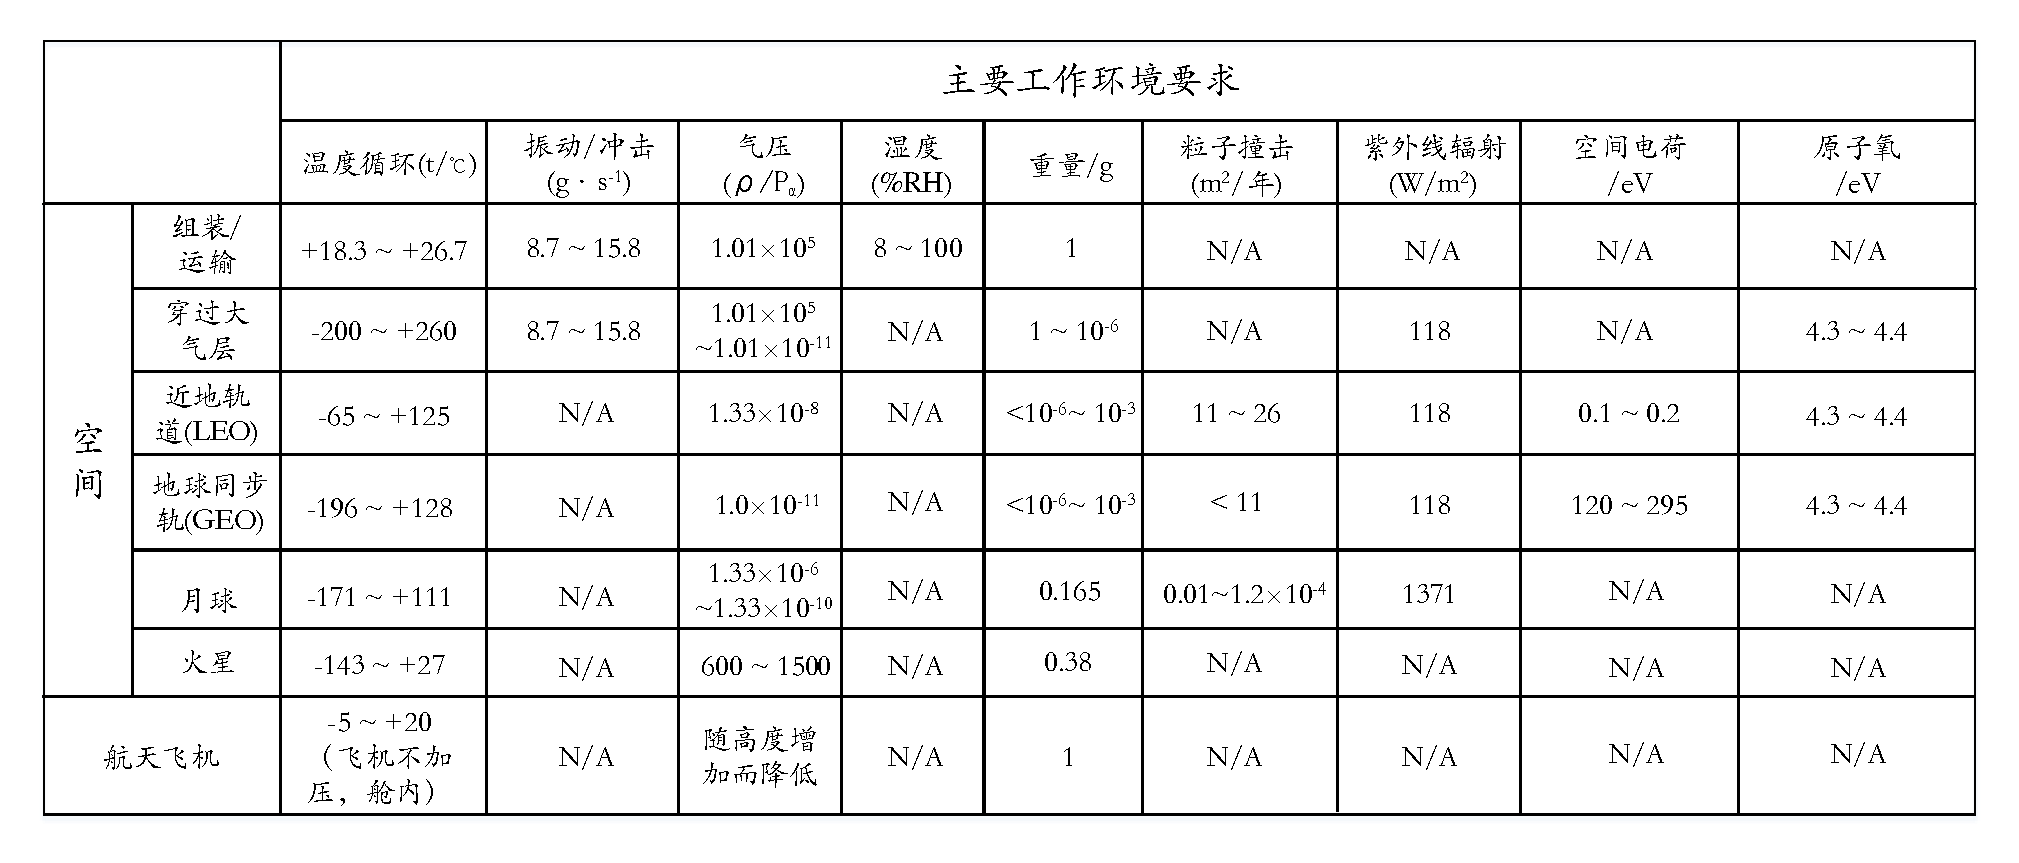
\includegraphics[width=15cm,height=7cm]{AeroEnviron.pdf}\\
\iffalse
\begin{tabular}{|c|c|c|c|c|}
\hline
\multirow{2}{*}{Multi-Row} &
\multicolumn{2}{c|}{Multi-Column} &
\multicolumn{2}{c|}{\multirow{2}{*}{Multi-Row and Col}} \\
\cline{2-3}
  & column-1 & column-2 & \multicolumn{2}{c|}{} \\
\hline
label-1 & label-2 & label-3 & label-4 & label-5 \\
\hline
\end{tabular}
\fi
\end{table}
%\fi
\subsection{极端温度环境}
\label{sub:chap2:temperature}
极端温度环境是影响电子元器件的主要原因之一\cite{Cressler2013Extreme},环境温度的变化会引起电子元件参数的浮动,从而影响电子电路的性能。对于有源器件,环境温度的升高会改变它固有的电学特性,导致漏电流增加。环境温度降低则漏电流减小。对于无源元件,由于封装采用的键合材料间的热膨胀系数~(CTE)~不同,极端温度会使得元器件的封装失效,引起电子元器件参数的变化。电子系统的极端温度工作环境主要可以分成三种情况:(1)~极端低温工作环境、(2)~极端高温工作环境、(3)~大范围温度变化工作环境。

\newpage
~(1)~极端低温工作环境

低于标准商业元件使用温度~$\left(0^ {\circ}C\backsim85^{\circ}C\right)$~或者在军事领域低于军事标准温度范围~$\left(-55^ {\circ}C\backsim125^{\circ}C\right)$~的工作环境被认为是极端低温工作环境\cite{Cressler2013Extreme}。许多行星表面都表现为极端低温环境,例如,在冬季火星表面温度可低至~$-143^ {\circ}C$。哈勃太空望远镜的继任者\raisebox{0.5mm}{------}詹姆斯$\cdot$韦伯~(James Webb)~太空望远镜~(JWST)~常年工作在~$-246^ {\circ}C$~左右的外太空,其搭载的电子设备与控制系统也都处于极端低温工作环境中\cite{Lightsey2004Optical}。由于晶体管的噪音干扰与环境温度成线性正相关,许多电子仪表设备为了提高系统精度都要工作在低温环境中。极端低温的工作环境也常见于医疗图像系统,卫星接收机以及高性能计算机系统之中。

~(2)~极端高温工作环境

高于标准商业元件使用温度~$\left(0^ {\circ}C\backsim85^{\circ}C\right)$~或者在军事领域高于军事标准温度范围~$\left(-55^ {\circ}C\backsim125^{\circ}C\right)$~的工作环境被认为是极端高温工作环境\cite{Cressler2013Extreme}。航空航天推动引擎电子系统经常需要工作在~$200^ {\circ}C\backsim300^{\circ}C$,一些特定的太空探索任务也需要工作在极端高温环境中,例如金星表面的温度可以高达~$600^ {\circ}C$。除了航空航天领域外,汽车电子设备、大型能源开采装置如石油、天然气钻井以及大型发电厂中的电子设备也都长期工作在极端高温环境中\cite{Johnson2002High}。

~(3)~大范围温度变化工作环境

从电子电路及电子元件封装的可靠性来看,相对于长时间工作在极端高温或极端低温的工作环境中,环境温度短时间内在极端低温与极端高温之间循环摆动的情况对电路的性能以及元器件的参数带来更大的挑战。这种大范围温度变化的工作环境常见于航空航天领域,例如在月球表面\cite{Jaeger1953Conduction},暴露在太阳光下的区域温度最高可达到~$120^{\circ}C$,而在月球背面的盆地处温度最低可达~$-230^{\circ}C$。这样超过~$300^{\circ}C$~的大范围温度变化随着月球的自转每~28~天循环一次,这样极端的温度变化对在月球表面进行勘探的电子设备及控制系统的稳定性提出了苛刻的要求。

\subsection{极端辐射环境}
\label{sub:chap2:radiation}
工作在电磁辐射通量较大的电子电路,其电子元件中电荷载流子的定向移动会受到电磁辐射的影响,造成电子电路的参数错误或电子系统的严重故障\cite{Stassinopoulos1988Space,Li2005SpaceRadiation}。在太空中遍布着放射性的粒子,银河系中的宇宙射线~(GCR)~和太阳发出的辐射粒子使得宇宙空间的电磁辐射环境异常复杂。11~年一次的太阳风暴包含大量的高能~$\chi$~射线、伽马射线以及带电粒子\cite{Dodd2010Current},这样极端的粒子辐射环境对航空航天领域的电子设备提出了重大考验。电子系统的极端辐射环境也可以分成三种情况:(1)~总离子辐射量工作环境、(2)~单粒子效应工作环境、(3)~粒子位移损伤工作环境。

~(1)~总离子辐射量工作环境

当电离性射线长期照射电子元器件时,高能量光子与固体物质相互作用会造成半导体产生本征激发,即产生电子~-~空穴对,从而对电子元件造成电离损伤。放射性射线的总离子辐射量过大会造成航天器材料的机械性能下降、强度变坏,同时使得航天材料的光学、热学、电学等性能退化。实验表明\cite{Son2010GaN},未加屏蔽及任何防护措施的电子系统仅可工作在~10Mrad~的辐射环境下,通过增加屏蔽装置,可以提高电子系统承受辐射的能力。

~(2)~单粒子效应工作环境

单粒子效应主要体现在高能粒子或重离子穿过电子器件时对电子器件的伤害。宇宙射线和太阳离子可以通过电离作用产生足够多的自由电荷,当射线穿过电子元件时,沉淀在器件中的电荷被结电容或电极吸收,造成逻辑状态改变,这种现象被称为单粒子翻转~(SEU)~\cite{Lum2004New}。当重离子和高能粒子照射到~CMOS~内部寄生的~PN~结上,有可能产生~CMOS~本身所特有的“闩锁”现象~(SEL)~。若发生“闩锁”现象,只要不断电,~CMOS~元件就会持续通过大电流直至烧毁。而“闩锁”现象导致的大电流通过其他元器件,也会造成其他元件烧毁的事故,这种现象称为单粒子烧毁~(SEB)\cite{Sternberg2006Single}~。

~(3)~粒子位移损伤工作环境

当宇宙射线中包含大量高能量、大质量的粒子流,这些高能粒子可能会通过弹性碰撞~\raisebox{0.5mm}{------}~Rutherford~散射来使晶格母体原子偏离原来的晶格位置,造成晶格缺陷。对于~Si~晶体,产生一对间隙原子~-~空位需要的平均能量为~$15eV\sim40eV$。因此,能量大于~$170keV$~的电子束即可在半导体元件内部产生一系列间隙原子和空位,这种现象称为粒子位移损伤。若电子电路长时间暴露在高能量、大质量的粒子流射线中,将会导致电路中晶体管性能恶化,甚至出现永久故障。
\section{温度变化对电子元件的影响}
\label{sec:chap2:temp_ele}
\subsection{温度变化对电阻元件的影响}
由电阻产生的原理可知,当环境温度升高,导体内原子热振动的振幅增大,与定向移动的电荷载流子相碰的机会增多,即导体呈现的电阻值增大。相反,当环境温度降低,导体内原子热振动的振幅减小,与定向移动的电荷载流子碰撞的机会降低,导体呈现的电阻值降低。不同材料制作的电阻,其参数值随温度变化的趋势不同。在不同的环境温度下,电阻的具体参数值可以由式~\ref{equ:chap2:Index1}~得到。
\begin{equation}\label{equ:chap2:Index1}
  R_{tem}=R_{ref}\cdot\left[1+\alpha\cdot\left(T-T_{ref}\right)\right]
\end{equation}

%式中,$\lambda_{max}$~为判断矩阵的最大特征值
%\hspace{1.3cm}n为判断矩阵的阶数
式中,$R_{tem}$~~为受温度影响后的电阻值

\hspace{1.3cm}$R_{ref}$~~为电阻的标准参数

\hspace{1.3cm}$\alpha$~~~~~~为导体材料的电阻温度系数

\hspace{1.3cm}$T$~~~~~~为电阻实际工作温度

\hspace{1.3cm}$T_{ref}$ ~为电阻标准参数值的工作温度
\iffalse
\begin{table}[htbp]    %用表格的方式实现
      \begin{tabular}{C{1cm}p{0.5cm}p{7cm}}
                             & $R_{tem}$     &为受温度影响后的电阻值\\

                             & $R_{ref}$      & 为电阻的标准参数\\

                            & $\alpha$         &为导体材料的电阻温度系数\\

                            & $T$                 &为电阻实际工作温度\\

                            & $T_{ref}$       &为电阻标准参数值的工作温度\\
\end{tabular}
\end{table}
\fi
\subsection{温度变化对电容元件的影响}
电容元件是由被绝缘物质分开的一对金属板或电极所构成的,通过导体之间的电场来存储能量,其中的绝缘物质被称作电介质。
\begin{figure}[h]
  \centering
     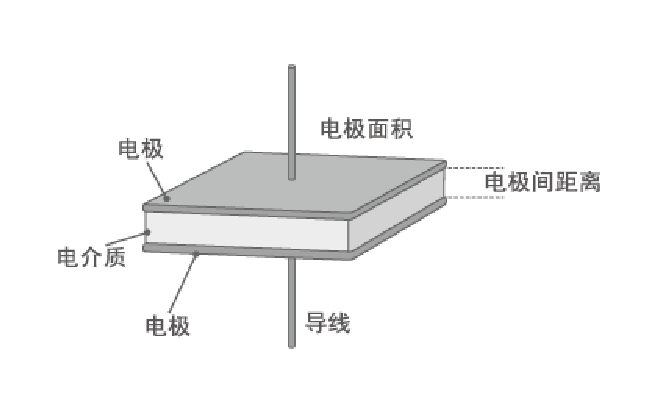
\includegraphics[width=8cm]{Capacitor.pdf}\\
   \caption{电容元件基本结构}\label{fig:chap2:capacitor}
\end{figure}

电容元件的电介质材料有许多种类,按照电介质的种类可以将电容分为电解电容、有机电容、无机电容以及超级电容四种类型。电容元件的电容值、耐压性能、介质常数、绝缘电阻以及电容对温度的敏感程度都取决于电介质的材料。

在常用的电容元件中,通用的陶瓷单片~Z5U~电容器由于其小尺寸与低成本的特点在电路中得到广泛应用,然而~Z5U~电容器的老化率最大可达到每~10~年下降~$5\%$~,因此不适用于高可靠的工业应用。被称为温度稳定型的陶瓷电容器~X7R~电容,在~$-55^{\circ}C$~到~$+125^{\circ}C$~的温度范围内,电容参数有~$15\%~$左右的非线性变化,主要用于要求不高的工业应用。~NPO~电容与~XHT~电容在温度稳定性、介质损耗以及元件可靠性方面性能较好,其中~NPO~电容是具有温度补偿特性的单片陶瓷电容器,在~$-55^{\circ}C$~到~$+125^{\circ}C$~的温度范围内电容参数的变化仅为~$30ppm/^{\circ}C$,随频率的变化也在~$\pm0.3\Delta C$~范围内\cite{Rito2013Communications}。但由于其内部填充电介质的特殊性,与其他电容相比~NPO~电容在相同的封装尺寸下电容参数有明显的限制,因此~NPO~电容常用于振荡器、谐振器的槽路电容以及高频电路中的耦合电容。XHT~电容虽然在温度稳定性方面略逊于~NPO~电容,但~XHT~电容在~$-55^{\circ}C$~到~$+125^{\circ}C$~的温度范围内也保持着~$5\%$~以内的电容值变化,同时由于电介质的高介电常数使得~XHT~电容元件的电容值是相同物理尺寸~NPO~电容的~10~倍。因此,本文中依据~XHT~电容元件的温度特性建立空间电源电容元器件的数学模型。

~Presidio~公司是一家长期制作高质量军用电子元件的公司,通过~Presidio~公司提供的~XHT~电容值随温度变化的曲线\cite{Presidio2016Electrical},读取~XHT~电容变化曲线上的数据并采用~MATLAB~软件中曲线拟合工具箱对数据进行拟合分析,采用多项式拟合的方式得到~XHT~随温度变化的函数表达式,建立空间电源电容元件随温度变化的数学模型。
\begin{figure}[h]
  \centering
     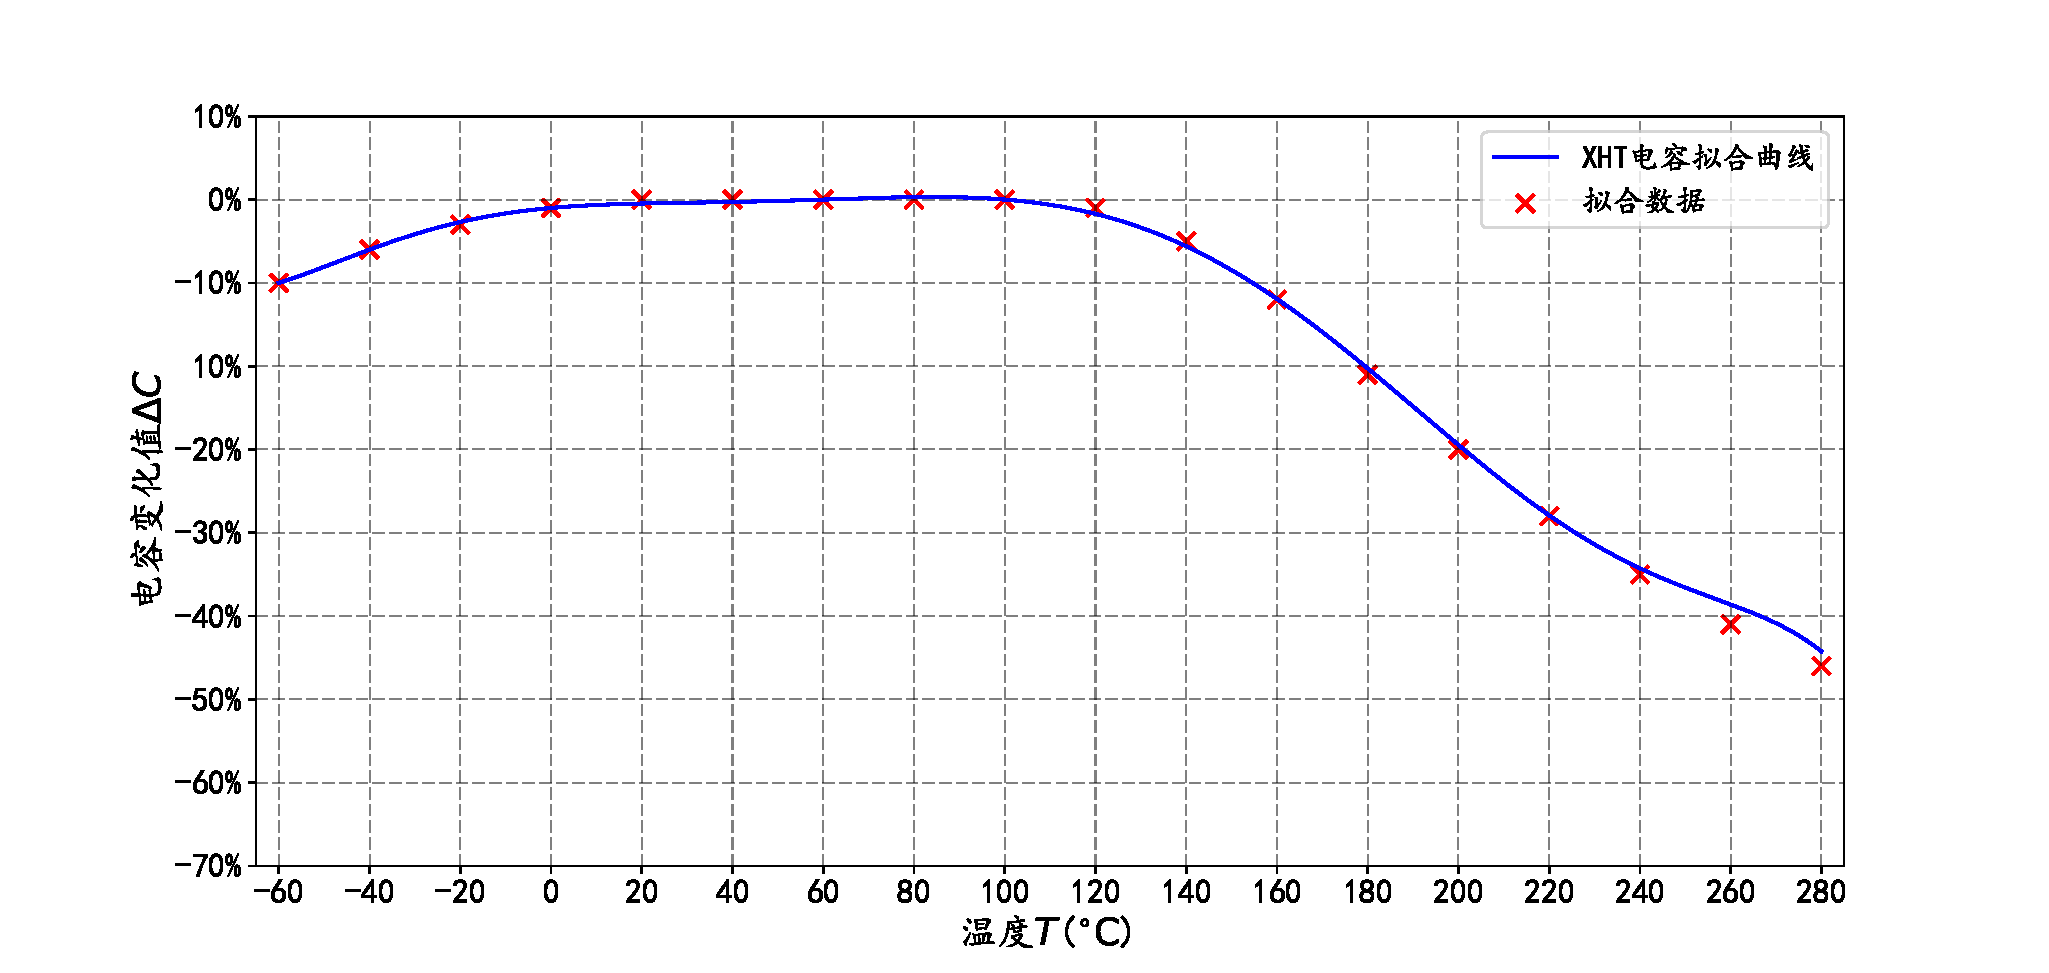
\includegraphics[width=14cm]{Capacitance-change.pdf}\\
   \caption{~XHT~电容随温度变化曲线}\label{fig:chap2:capacitance-change}
\end{figure}
\begin{equation}\label{equ:chap2:Index2}
  C_{tem}=C_{ref}\cdot\left(1+\Delta C\right)
\end{equation}

式中,$C_{tem}$~为受温度影响后的电容值

\hspace{1.3cm}$C_{ref}$~为电容的标准值

\hspace{1.3cm}$\Delta C$~~为电容由温度引起的变化值

由温度引起的电容值变化~$\Delta C$~为通过曲线拟合得到的关于环境温度~T~的多项式
\begin{equation}\label{equ:chap2:Index3}
  \Delta C=f\left(T\right)\times 100\%=p_1\cdot T^7+p_2\cdot T^6+p_3\cdot T^5+p_4\cdot T^4+p_5\cdot T^3+p_6\cdot T^2+p_7\cdot T+p_8
\end{equation}

多项式参数为

\qquad \qquad $p_1=-1.569\times 10^{-16}$     ~~~~~\qquad \qquad ~$p_5= 1.780\times 10^{-7} $

\qquad \qquad  $p_2= 1.085\times 10^{-13}$    ~~~~~\qquad \qquad ~~~$p_6=-1.461\times 10^{-5}$

\qquad \qquad $p_3=-2.215\times 10^{-11}$     ~~~~~\qquad \qquad $p_7= 0.487\times 10^{-4}$

\qquad \qquad $p_4= 5.817\times 10^{-10}$     ~~~~~\qquad \qquad ~~~$ p_8=-0.01$

\iffalse
\begin{table}[htbp]
  \centering
\begin{tabular}{p{5cm}p{5cm}}

  $p_1=-1.569\times 10^{-16}$     & $p_5= 1.780\times 10^{-7} $\\

  $p_2= 1.085\times 10^{-13}$     & $p_6=-1.461\times 10^{-5}$ \\

  $p_3=-2.215\times 10^{-11}$     & $p_7= 0.487\times 10^{-4}$ \\

 $p_4= 5.817\times 10^{-10}$      & $ p_8=-0.01$ \\

\end{tabular}
\end{table}
\fi
曲线的参数指标为

\qquad  误差平方和~$SSE\colon~~3.55\times10^{-4}$  ~\qquad   均方差~$MSE\colon~~1.97\times10^{-5} $

\qquad 均方根~$RMSE\colon~~~5.96\times10^{-3}$    ~~~~~\qquad 确定系数~$R-square\colon~~0.9995$

\subsection{温度变化对电感元件的影响}
电感元件是通过电磁感应工作的电子元件,电感绕线的材质、绕制圈数、绕线方式、线径、磁芯结构等都会影响电感元件的参数值。当电感元件根据标准的加工流程制作出来后,在实际使用过程中,电感元件主要受到工作环境的温度和湿度影响。由于电感线圈导线受热作用后膨胀会产生几何变形,因此在不同工作温度中电感的参数会产生差异。通常用电感的稳定性来描述这一特征\cite{Wang2006Electronic},定义电感温度系数~$a_{L}$~为
\begin{equation}\label{equ:chap2:Index4}
a_L=\FS{L_2-L_1}{L_1\cdot\left(T_2-T_1\right)}~~~~\left(1/^{\circ}C\right)
\end{equation}

式中,$L_1$~和~$L_2$~分别表示~$T_1$~和~$T_2$~环境温度下的电感参数值~(H)~,通常用电感温度系数~$a_L$~来衡量电感元件的稳定程度。对于湿度的影响,一般在制作电感元件时采用环氧树脂封装或浸渍处理来防止湿度造成的参数值变化\cite{Dong2006Sensor}。本文中电感元件的参数值~$L_{tem}$~随温度变化的数学模型为
\begin{equation}\label{equ:chap2:Index5}
L_{tem}=L_{ref}\cdot\left[a_L\cdot\left(T-T_{ref}\right)+1\right]
\end{equation}

式中, $L_{tem}$ ~为受温度影响后的电感值

\hspace{1.3cm}$L_{ref}$ ~~为电感的标准值

\hspace{1.3cm}$a_L$\ ~~~~~为电感的温度系数

\hspace{1.3cm}$T$  \ ~~~~~为电感实际工作温度

\hspace{1.3cm}$T_{ref}$ ~~为电感标准参数值的工作温度
\section{辐射对电子元件的影响}
\label{sec:chap2:radia_ele}
鉴于航空航天领域复杂的辐射环境,航空航天领域电子系统中所用的电子器件都采用了抗辐射加固技术,确保电子系统、仪器等在辐射环境中能够完好可靠地工作。航空领域半导体分立元件的封装都经过特殊设计,使得管壳与管芯间保持高真空或填充适当的填充材料,从而抵抗辐射对元器件的影响。在电路设计方面通常也会设计各种补偿电路,如达林顿电路,集电极阻抗补偿电路、晶体管对电路,用来补偿粒子辐射引起的增益下降、瞬时光电流等现象。由于专为高可靠环境设计制造的元器件成本较高,对于大量应用的无源元器件,为实现“更快、更好、更便宜”的目的,航空航天项目中普遍采用商业级~(COTS)~元器件来替代特殊设计元件,如国际空间站~(ISS)~的~EXPRESS~(Expedite the Processing of Experiments to Space Station Rack)~项目,已将商业级~(COTS)~元器件应用于高可靠的航天环境中\cite{Cook2013Capabilities}。

目前,辐射对电子元件影响的研究成果主要集中在~MOSFET~及半导体二极管等有源元件以及由它们所构成的复杂电路领域,对于无源元件电阻、电容及电感的研究较少。因此,为了建立空间电源电子元件的数学模型,本文详细研究了辐射对无源元件电阻、电容及电感的影响。
\subsection{辐射对电阻元件的影响}
从广义上来说,无源元器件并不像有源元件那样易受到总离子辐射量的影响,原因在于无源元件内部没有对氧化层损失敏感的区域。但在强烈的离子辐射环境下,无源元件的参数值还是会有微小的变化。

分析辐射对无源元件的影响最直接的方式就是将无源元件暴露在极端辐射环境中,经过一段时间后测量无源元件参数的变化量。离子辐射的测量采用单位拉德~(rad),1 rad~是指~1 g~受照射的物质吸收任何一种射线~100 erg~(尔格)~辐射能时的辐射剂量~$(1rad=0.01J/kg)$~。对于电阻元件,~Wilcox~等人在~UC~Davis~Croker~核能实验室中对强辐射航天环境中电子元件进行了辐射实验\cite{Wilcox2010Silicon},将一系列不同封装的电阻暴露在~1Mrad~的质子辐射环境中,实验表明~4~种常见封装的电阻在不同电路结构下,电阻的阻值都有微小的变化,但变化范围不超过原电阻参数值的~$2\%$~,实验结果如图~\ref{fig:chap2:radia-r1}~所示。

在~1991~年美国国家核安全局下属的桑迪亚国家实验室~(Sandia National Laboratories),C.L.Axness、L.Riewe~等人对半绝缘多晶硅型~(SIPOS)~及多晶硅电阻进行了辐射实验\cite{Axness1991Radiation},在辐射环境由~0 rad~变化到~$1\times 10^7rad$~的过程中记录电阻值参数的变化。由图~\ref{fig:chap2:radia-r2}~可以看出,辐射环境从~0 rad~变化到~$1\times 10^7rad$~的过程中,电阻参数仅有微小的变化,与~Wilcox~等人的实验结果相近。通过分析~Wilcox~以及~C.L.Axness~等人的实验结果,将受到~1~Mrad~质子辐射后,4~种封装的电阻元件在~8~种不同电路结构中的参数变化取均值可得,经过~1Mrad~质子辐射后电阻参数值比辐射前增加了~$0.86\%$。因此,在航空航天极端辐射环境中的电阻元件参数~$R_{rad}$~可以描述为
\begin{equation}\label{equ:chap2:Index6}
  R_{rad}=1.0086\times R
\end{equation}

式中,  $R_{rad}$  ~~为极端辐射环境中的电阻元件参数

\hspace{1.3cm}~$R$ ~\quad ~为受辐射前,电阻元件的参数

\begin{figure}[h]
  \centering
     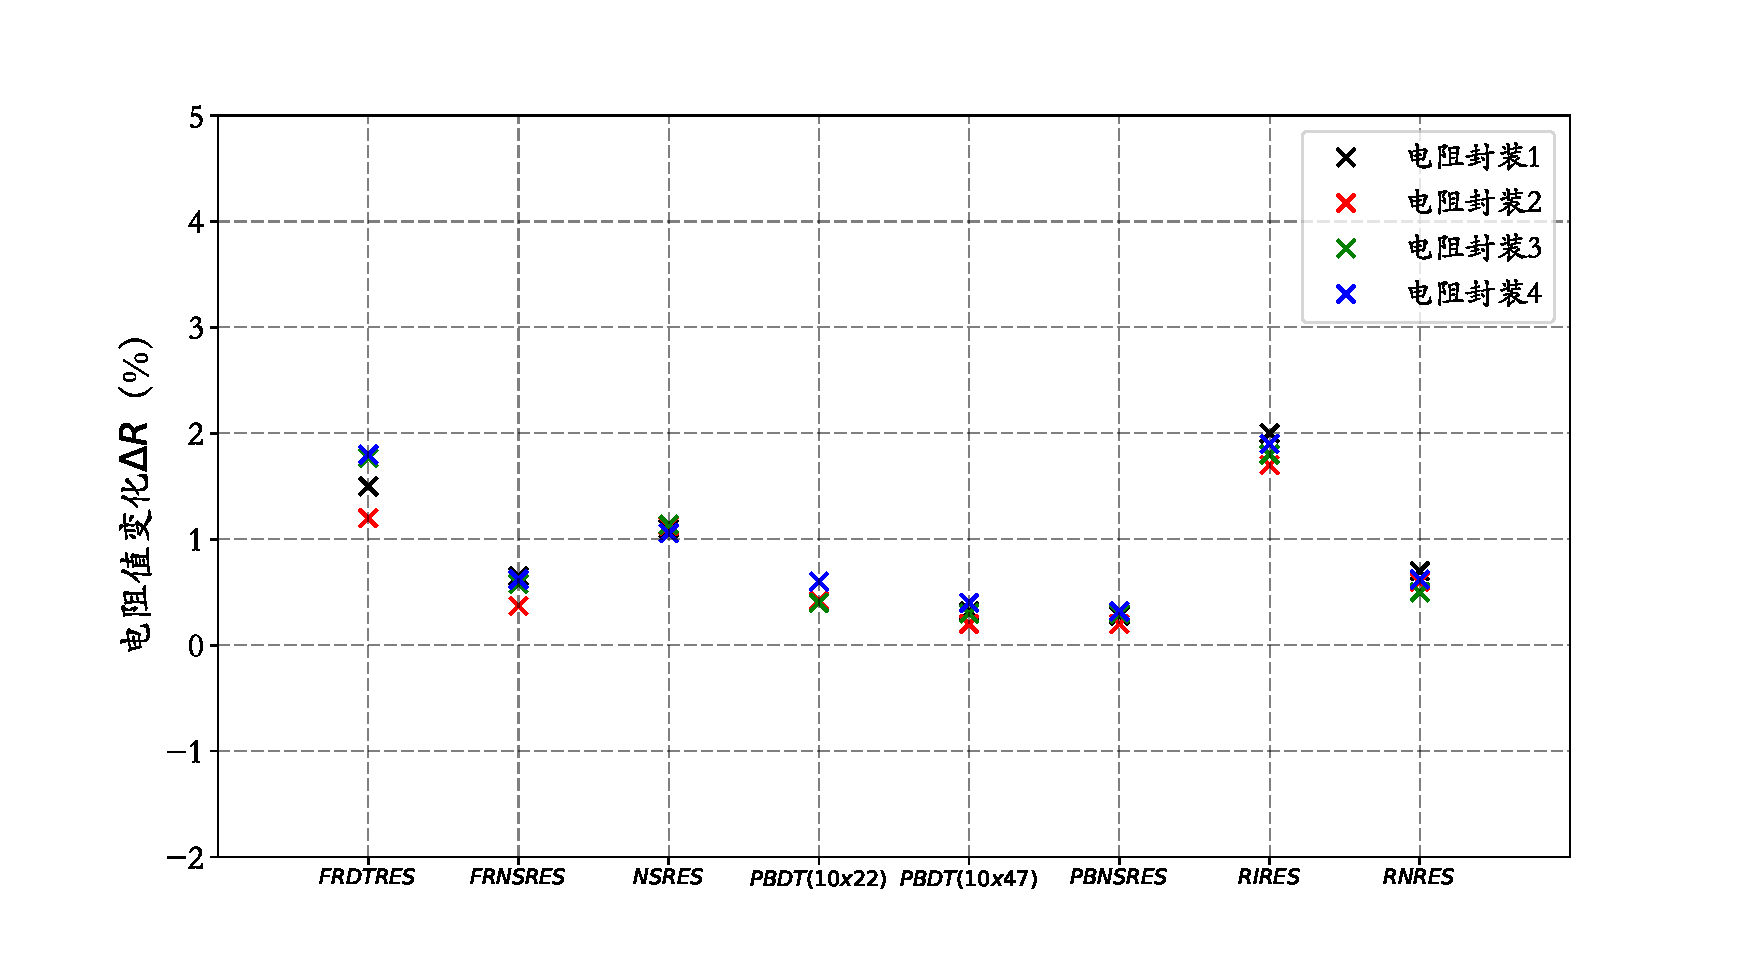
\includegraphics[width=12cm]{Radia-R1.pdf}\\
   \caption{极端辐射环境中四种不同封装电阻
在~8~种电路结构中参数值的变化}\label{fig:chap2:radia-r1}
\end{figure}
\begin{figure}[h]
  \centering
     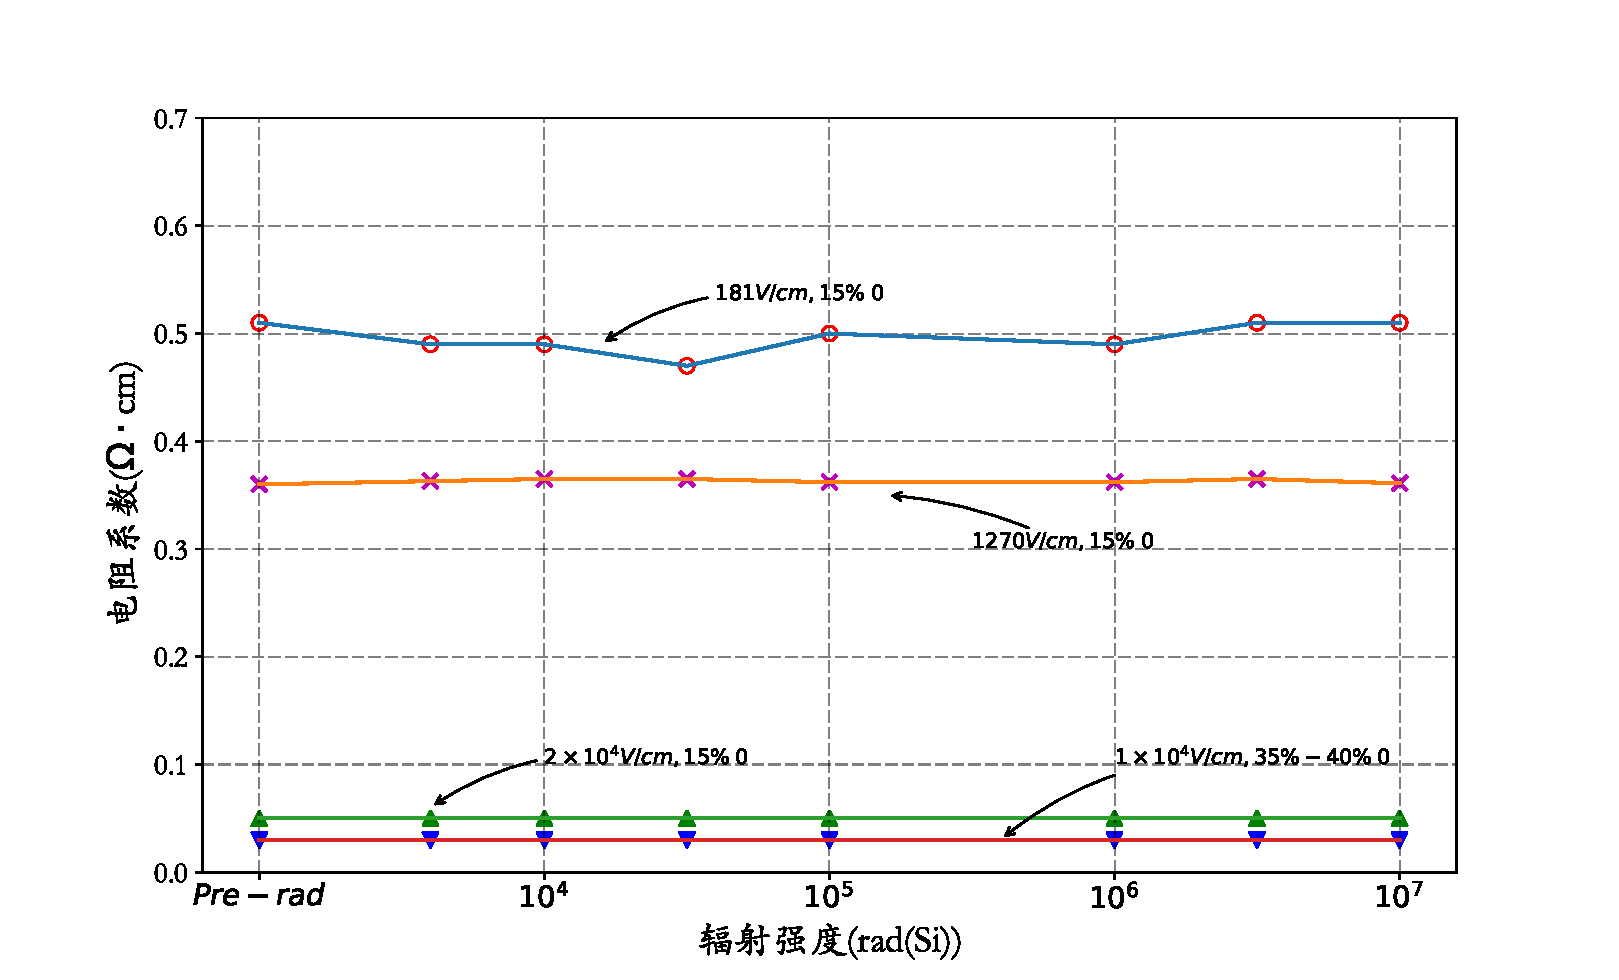
\includegraphics[width=12cm]{Radia-R2.pdf}\\
   \caption{半隔离多晶硅型及无隔离多晶硅电阻在辐射环境中电阻系数的变化}\label{fig:chap2:radia-r2}
\end{figure}
\subsection{辐射对电容元件的影响}
由于电容元件的值依赖于两个电极之间存储电荷量的关系,相比于电阻更容易受到电磁辐射的影响。英国布鲁内尔大学的~Ignacio Yaselli~等人研究了工作在强烈的电磁辐射中~HV~滤波器电路中电容元件参数值的变化\cite{Yaselli2008Studying}。Ignacio Yaselli~等人通过分析~Premier Farnell~公司~1 nF - 2 kV~的电容元件在不同辐射环境中元件参数值的变化,来预测在恶劣辐射环境中电容参数值以及~HV~滤波器性能的变化。在~Ignacio~的文章中,通过放射钴~60(Cobalt - 60)~射线来模拟太空环境中的辐射环境,在实验中采用~Gy~作为表征辐射的单位。与~rad~一样,Gy~也是一种国际常用的辐射单位,度量的是~1 kg~被辐射物质吸收~1~焦耳的能量,与~rad~的换算公式如下。
\begin{equation}\label{equ:chap2:Index7}
  1Gy=1J/kg=100rad
\end{equation}

为保证实验的测试结果能够反映辐射对电容产生的普遍影响,在实验中对~10~个完全相同的~1 nF - 2 kV~电容元件每一个电容进行~10~次辐射实验,从而分析辐射对电容元件参数的影响。Ignacio~等人分别在没有辐射的环境、25.9 kGy~辐射环境以及~345 kGy~辐射环境中对电容元件进行辐射实验。其中~345 kGy~的辐射环境是模拟电容元件在太空中工作~10~年后的状态,实验数据曲线如图~\ref{fig:chap2:cap-345kgy}~所示。
\begin{figure}[h]
  \centering
     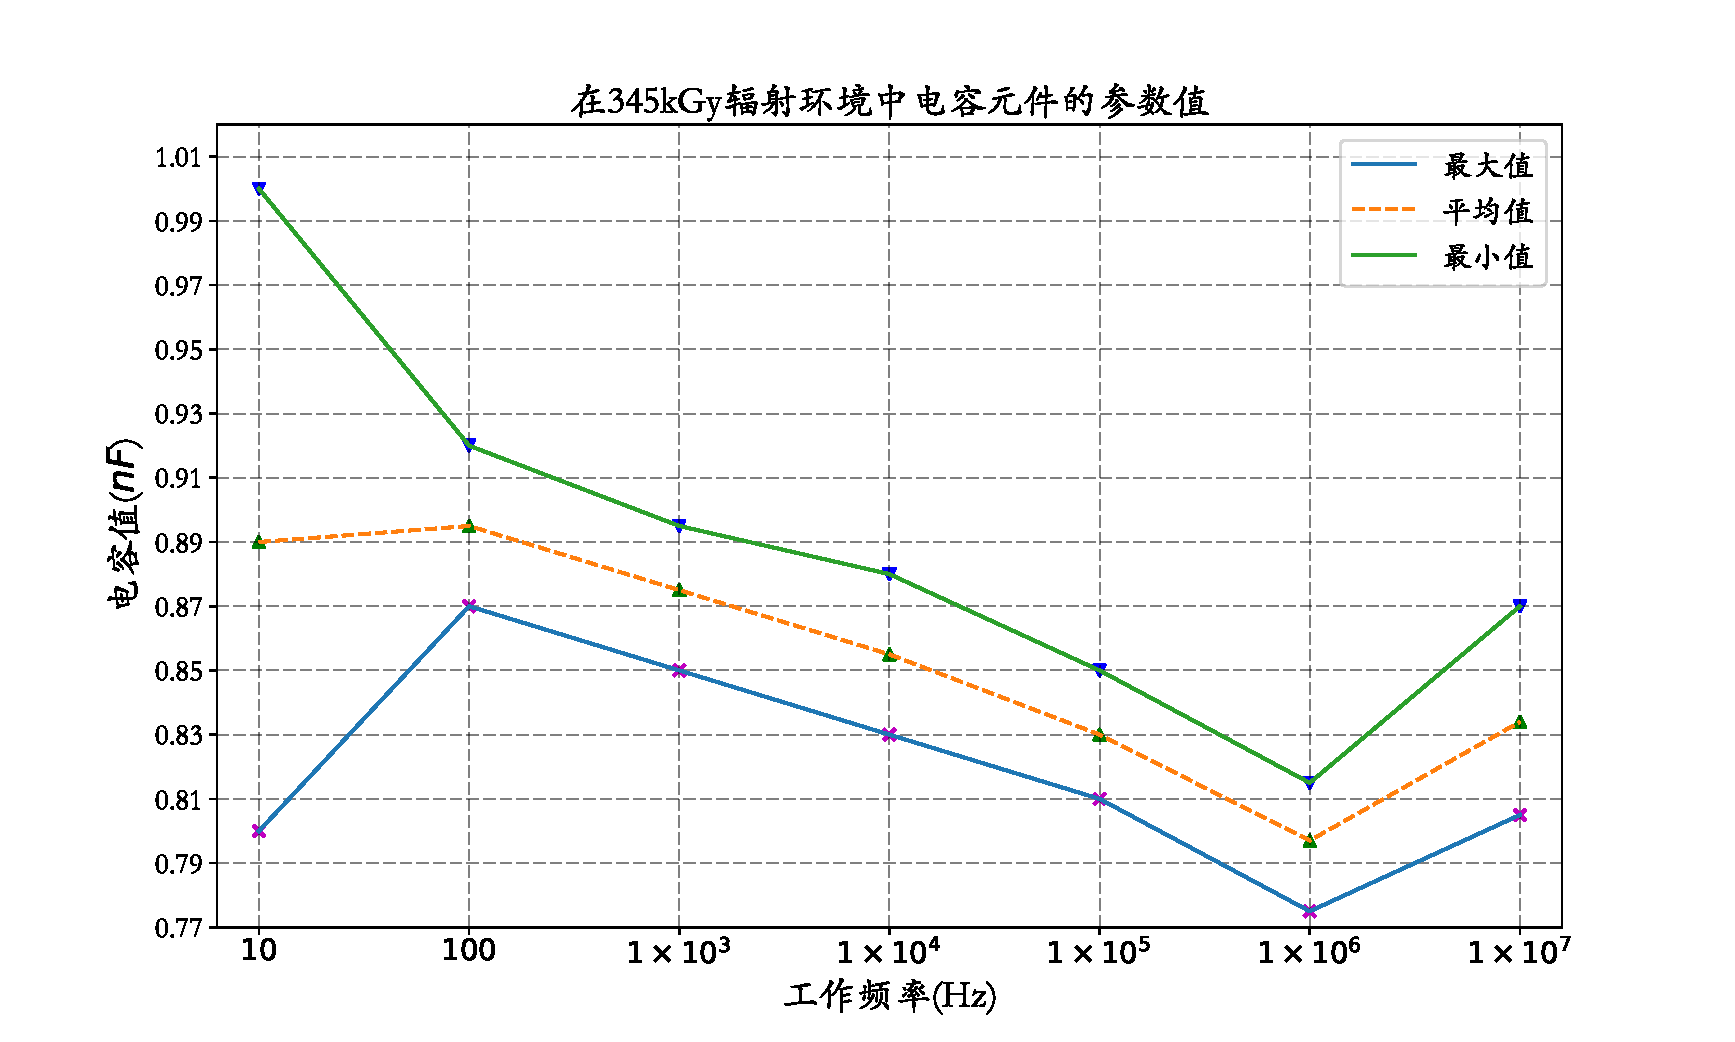
\includegraphics[width=13cm]{Cap-345kgy.pdf}\\
   \caption{辐射环境中~1nF 2kV~电容元件参数变化}\label{fig:chap2:cap-345kgy}
\end{figure}

由实验结果可知在~25.9 kGy~的辐射环境中,不同工作频率下电容元件的参数值基本相同,25.9 kGy~的辐射对电容元件并没有显著的影响。而由图~\ref{fig:chap2:cap-345kgy}~可知,在~345 kGy~的辐射环境中电容参数与电磁辐射前相比有明显的下降。在~10Hz~的低频工作状态中,辐射环境中的电容参数下降~$10\%$~左右,在高频时辐射环境中电容元件参数普遍下降~$5\%$。

由于开关式电源电路通常工作在~100 kHz~的频率附近,因此根据~100 kHz~工作频率下电容元件在~345 kGy~辐射环境中参数的变化来对极端辐射环境中电容元件参数~$C_{rad}$~进行建模。
\begin{equation}\label{equ:chap2:Index8}
  C_{rad}=0.83\times C
\end{equation}

式中,  $C_{rad}$  ~为极端辐射环境中的电容元件参数

\hspace{1.4cm}$C$  \quad ~为受辐射前,电容元件的参数
\subsection{辐射对电感元件的影响}
对于电感元件在极端辐射环境中参数的变化,Cressler~与~Hamilton~等人对无源~LC~滤波器电路进行了离子辐射实验\cite{Cressler2001Proton}。在离子能量密度高达 ~$5\times 10^{13}p/cm^2$~的辐射环境下,对~LC~滤波器的各项参数进行检查并与辐射实验前的各项数据相比较,实验的具体参数值如表~\ref{tab:chap2:radia-exper}~所示。
\begin{table}[htbp]
  \centering  \caption{~LC~滤波器在辐射实验前后的参数对比}
  \label{tab:chap2:radia-exper}
\begin{tabular}{C{4cm}C{2cm}C{5cm}C{2cm}}
\toprule
  参数                                            &辐射前        &$5\times 10^{13}p/cm^2$~辐射环境中      &单位\\
\midrule
 滤波器的品质因数 Q                 &7.6               &7.6                                                                & -       \\

          插入损耗                            &16.8             &16.8                                                             & dB     \\

            电感值                              &2.5               &2.5                                                                & nH    \\

      电感品质因数                        &7.4               &7.4                                                                & -       \\
\bottomrule
\end{tabular}
\end{table}

由实验数据可以看出,$5\times 10^{13}p/cm^2$~离子能量密度的辐射环境并没有对~LC~滤波器造成明显的影响,电感值与品质因数都与辐射实验前相同。离子辐射对~LC~滤波电路的影响在频域响应曲线中有所体现,从~LC~滤波电路实验前后的频域响应对比曲线可知,在低频段辐射对~LC~滤波电路并没有明显的影响,但在高频段经过辐射的~LC~滤波电路频域响应曲线有微小的偏移\cite{Cressler2001Proton}。

Michelis~与~Faccio~等人通过优化~PCB~电路板的布局,将电磁辐射能够影响到的电感部分压缩到最低\cite{Michelis2008Air}。通过强烈的辐射实验测试,电感参数始终没有明显的变化,经过设计优化后的空芯电感在极端辐射环境中十分接近理想的、不受电磁辐射干扰的、无损耗的电感。
\newpage
\begin{figure}[h]
\begin{minipage}[t]{0.5\linewidth}
  \centering
  % Requires \usepackage{graphicx}
  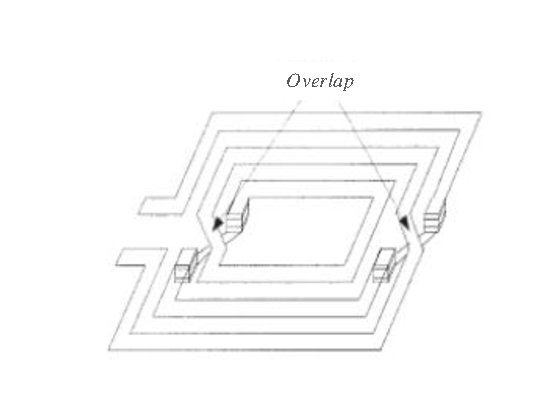
\includegraphics[height=5cm]{L-layout.pdf}\\
  \caption{对称螺旋式空芯电感布局}\label{fig:chap2:l-layout}
\end{minipage}
\begin{minipage}[t]{0.5\linewidth}
  \centering
  % Requires \usepackage{graphicx}
  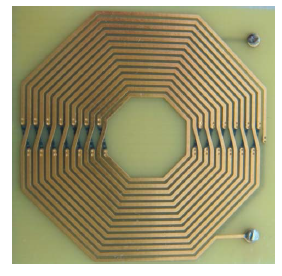
\includegraphics[height=5cm]{L-reality.png}\\
  \caption{对称螺旋式空芯电感实物}\label{fig:chap2:l-reality}
\end{minipage}
\end{figure}

根据上述文献资料与分析可以得知,极端辐射环境对电感元件的各项参数影响不大,且通过适当的优化设计,在极端辐射环境中工作的电感十分接近理想的电感元件。因此,本文在建立极端环境下空间电源电路电子元器件的数学模型时,不考虑辐射对电感元件产生的影响。
\section{空间电源电子元器件退化模型的建立}
\label{sec:chap2:mathematic-model}
根据本章之前的分析,建立空间电源电子元器件退化模型需要考虑极端温度环境与极端辐射环境两方面因素。由于空间电源长时间工作在极端辐射环境中,而环境温度却在实时的变化。因此在建立空间电源电子元件的数学模型时,主要根据电子元件随环境温度变化的趋势描绘元件的退化模型,并以系数的方式将极端辐射环境对电子元件的影响反映在元件的退化模型中。
\subsection{空间电源电阻退化模型}
对于电路系统中普遍使用的铜制电阻,电阻温度系数~$\alpha$~为~0.00393,采用工作在~$20^{\circ}C$~下的电阻值作为标准电阻值,可得电阻元件随温度的变化趋势为
\begin{equation}\label{equ:chap2:Index9}
  R_{tem}=R_{ref}\cdot \left[1+0.00393\cdot \left(T-20\right)\right]
\end{equation}

考虑到极端辐射环境对电阻元件的影响,本文中空间电源电阻元件的退化模型为
\begin{equation}\label{equ:chap2:Index10}
  R=1.0086\cdot R_{ref}\cdot \left[1+0.00393\cdot \left(T-20\right)\right]
\end{equation}

式中,  $R$ ~\quad  为电阻的实际参数

\hspace{1.3cm}$R_{ref}$ ~为电阻的标准参数

\hspace{1.3cm}$T$ \quad ~为空间电源的工作温度
\subsection{空间电源电感退化模型}
电感元件的温度系数一般在~$25\sim125ppm/^{\circ}C$,本文中选用温度系数为~$88ppm/^{\circ}C$~的铜制电感线圈来建立空间电源电感元件的数学模型。同样以工作在~$20^{\circ}C$~温度下的电感参数作为标准电感值,则可得电感元件随温度的变化趋势为
\begin{equation}\label{equ:chap2:Index11}
  L_{tem}=L_{ref}\cdot \left[1+88\times 10^{-6}\cdot \left(T-20\right)\right]
\end{equation}

由于高强度的粒子辐射实验结果显示辐射环境对电感元件参数并没有显著的影响,并且通过设计电感的磁芯与优化~PCB~电路布局,可以在辐射环境中制作出近似理想的电感元件。因此在建立空间电源电感元件的退化模型时,忽略辐射对电感元件参数的影响,即本文中空间电源电感元件的退化模型为
\begin{equation}\label{equ:chap2:Index12}
  L=L_{ref}\cdot \left[1+88\times 10^{-6}\cdot \left(T-20\right)\right]
\end{equation}

式中,$L$~~~\quad 为电感的实际参数

\hspace{1.3cm}$L_{ref}$  ~为电感的标准参数

\hspace{1.3cm}$T$ ~\quad 为空间电源的工作温度
\subsection{空间电源电容退化模型}
对空间电源电容元件建立数学模型时,同样将~$20^{\circ}C$~温度下的电容元件参数值作为标准电容值,根据~Presidio~公司提供的~XHT~电容值随温度变化曲线来描述电容元件参数的变化趋势,考虑到极端辐射环境对电容元件参数的影响,本文所建立的空间电源电容元件的退化模型为
\begin{equation}\label{equ:chap2:Index13}
  C=0.83\times C_{ref}\cdot\left(1+\Delta C\right)
\end{equation}

式中,$C$~~~~~~~为电容的实际参数

\hspace{1.3cm}$C_{ref}$ ~~为电容的标准参数

\hspace{1.3cm}$\Delta C$\quad 为由温度引起的电容变化值,由多项式表示
 \begin{equation}\label{equ:chap2:Index14}
  \Delta C=f\left(T\right)\times 100\%=p_1\cdot T^7+p_2\cdot T^6+p_3\cdot T^5+p_4\cdot T^4+p_5\cdot T^3+p_6\cdot T^2+p_7\cdot T+p_8
\end{equation}	

多项式参数为

\qquad \qquad $p_1=-1.569\times 10^{-16}$     \qquad \qquad ~$p_5= 1.780\times 10^{-7} $

\qquad \qquad  $p_2= 1.085\times 10^{-13}$    \qquad \qquad ~~~$p_6=-1.461\times 10^{-5}$

\qquad \qquad $p_3=-2.215\times 10^{-11}$     \qquad \qquad $p_7= 0.487\times 10^{-4}$

\qquad \qquad $p_4= 5.817\times 10^{-10}$     \qquad \qquad ~~~$ p_8=-0.01$
\iffalse
\begin{table}[htbp]
  \centering
\begin{tabular}{p{5cm}p{5cm}}

  $p_1=-1.569\times 10^{-16}$     & $p_5= 1.780\times 10^{-7} $\\

  $p_2= 1.085\times 10^{-13}$     & $p_6=-1.461\times 10^{-5}$ \\

  $p_3=-2.215\times 10^{-11}$     & $p_7= 0.487\times 10^{-4}$ \\

 $p_4= 5.817\times 10^{-10}$      & $ p_8=-0.01$ \\

\end{tabular}
\end{table}
\fi
%%%%%%%%%%%%%%%%%%%%%%%%%%%%%%%%%%%%%%%%%%%%%%%%%%%%%%%%%%%%%%%
\section{本章小结}
\label{sec:chap2:sum}
本章围绕电子元器件的数学模型展开讨论。首先,由于理论分析是基于对实际物理模型的抽象描述这一事实,明确了研究空间电源在极端工作环境中电子元器件实际退化模型的必要性。通过分析航空航天高可靠应用领域的各项环境参数,将极端工作环境具体化为极端温度环境和极端辐射环境,从这两方面分析研究电阻、电容与电感参数的变化趋势。

然后通过查阅文献资料,研究了极端温度与极端辐射环境对不同材质电阻、电容及电感元件参数的影响。鉴于空间电源长时间工作在极端辐射环境中,在建立空间电源电子元件的数学模型时,根据电子元件的温度敏感性描绘元件参数的退化趋势,并以系数的方式反映辐射环境对元器件参数的影响。最后,根据以上研究内容,建立了科学的空间电源电子元件的量化数学模型,为后文中空间电源脆弱性分析与量化评估奠定基础。

%V/cm为电压梯度,是一种在电路中测量电阻变化的方式。

